% https://www.overleaf.com/
\documentclass[tikz,border=20pt]{standalone}
\usepackage{tikz}
\usepackage{amsmath}
\usepackage{array}
\usetikzlibrary{positioning, fit, arrows.meta}

\begin{document}

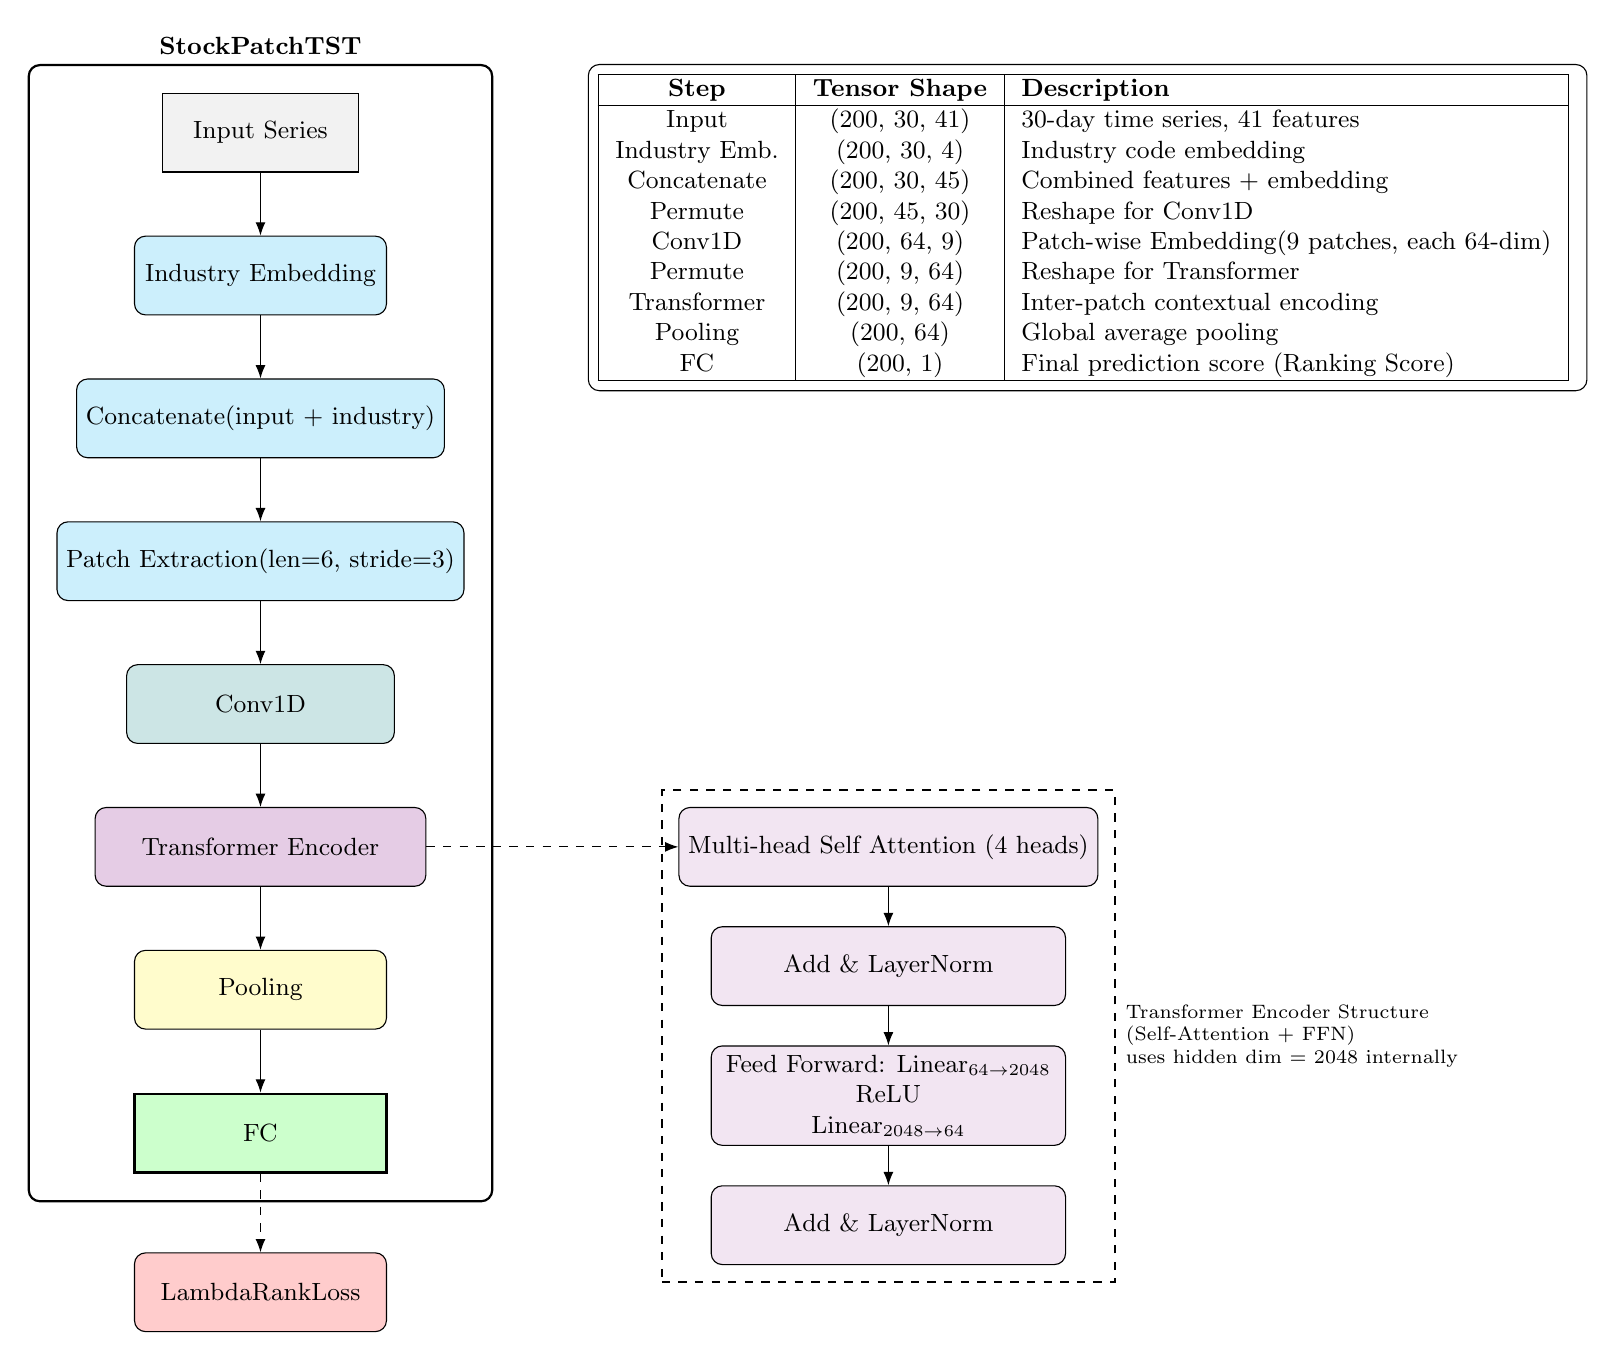
\begin{tikzpicture}[
    node distance=1cm and 1.2cm,
    every node/.style={font=\small},
    input/.style={rectangle, draw, minimum width=2.5cm, minimum height=1cm, fill=gray!10},
    embed/.style={rectangle, draw, rounded corners, minimum width=3.2cm, minimum height=1cm, fill=cyan!20},
    preprocess/.style={rectangle, draw, rounded corners, minimum width=3.2cm, minimum height=1cm, fill=cyan!20},
    conv/.style={rectangle, draw, rounded corners, minimum width=3.4cm, minimum height=1cm, fill=teal!20},
    transformer/.style={rectangle, draw, rounded corners, minimum width=4.2cm, minimum height=1cm, fill=violet!20},
    subblock/.style={rectangle, draw, rounded corners, minimum width=4.5cm, minimum height=1cm, fill=violet!10},
    pooling/.style={rectangle, draw, rounded corners, minimum width=3.2cm, minimum height=1cm, fill=yellow!20},
    output/.style={rectangle, draw, thick, minimum width=3.2cm, minimum height=1cm, fill=green!20},
    loss/.style={rectangle, draw, rounded corners, minimum width=3.2cm, minimum height=1cm, fill=red!20},
    arrow/.style={-Latex}
]

% Main model nodes (left)
\node[input] (input) {Input Series};
\node[embed, below=0.8cm of input] (embed) {Industry Embedding};
\node[preprocess, below=0.8cm of embed] (concat) {Concatenate\\(input + industry)};
\node[preprocess, below=0.8cm of concat] (patch) {Patch Extraction\\(len=6, stride=3)};
\node[conv, below=0.8cm of patch] (conv) {Conv1D};
\node[transformer, below=0.8cm of conv] (encoder) {Transformer Encoder};
\node[pooling, below=0.8cm of encoder] (pooling) {Pooling};
\node[output, below=0.8cm of pooling] (fc) {FC};
\node[loss, below=1.0cm of fc] (loss) {LambdaRankLoss};

% Arrows
\draw[arrow] (input) -- (embed);
\draw[arrow] (embed) -- (concat);
\draw[arrow] (concat) -- (patch);
\draw[arrow] (patch) -- (conv);
\draw[arrow] (conv) -- (encoder);
\draw[arrow] (encoder) -- (pooling);
\draw[arrow] (pooling) -- (fc);
\draw[arrow, dashed] (fc) -- (loss);

% 전체 테두리
\node[draw=black, thick, rounded corners, fit=(input)(embed)(concat)(patch)(conv)(encoder)(pooling)(fc), inner sep=10pt, label=above:{\textbf{StockPatchTST}}] (modelbox) {};

% Transformer 내부 구조 (오른쪽 확대)
\node[subblock, right=3.2cm of encoder] (mhsa) {Multi-head Self Attention (4 heads)};
\node[subblock, below=0.5cm of mhsa] (addnorm1) {Add \& LayerNorm};
\node[subblock, align=center, below=0.5cm of addnorm1] (ffn) {Feed Forward: Linear$_{64 \rightarrow 2048}$ \\ ReLU \\ Linear$_{2048 \rightarrow 64}$};
\node[subblock, below=0.5cm of ffn] (addnorm2) {Add \& LayerNorm};
\draw[arrow] (mhsa) -- (addnorm1);
\draw[arrow] (addnorm1) -- (ffn);
\draw[arrow] (ffn) -- (addnorm2);
\draw[arrow, dashed] (encoder.east) -- ++(0.4, 0) |- (mhsa.west);

\node[draw, thick, dashed, fit=(mhsa)(addnorm1)(ffn)(addnorm2), inner sep=6pt,
label=right:{\parbox{5cm}{\scriptsize Transformer Encoder Structure \\ (Self-Attention + FFN) \\ uses hidden dim = 2048 internally}}] {};

% 오른쪽 표: Tensor Shapes
\node[rectangle, draw, rounded corners, fill=white, align=left, above right=0cm and 1.2cm of modelbox.north east, anchor=north west] (tensor_table) {
    \begin{tabular}{|c|c|l|}
    \hline
    \textbf{Step} & \textbf{Tensor Shape} & \textbf{Description} \\
    \hline
    Input & (200, 30, 41) & 30-day time series, 41 features \\
    Industry Emb. & (200, 30, 4) & Industry code embedding \\
    Concatenate & (200, 30, 45) & Combined features + embedding \\
    Permute & (200, 45, 30) & Reshape for Conv1D \\
    Conv1D & (200, 64, 9) & Patch-wise Embedding(9 patches, each 64-dim) \\
    Permute & (200, 9, 64) & Reshape for Transformer \\
    Transformer & (200, 9, 64) & Inter-patch contextual encoding \\
    Pooling & (200, 64) & Global average pooling \\
    FC & (200, 1) & Final prediction score (Ranking Score) \\
    \hline
    \end{tabular}
};

\end{tikzpicture}

\end{document}
